\documentclass[conference, onecolumn]{IEEEtran}

\usepackage[utf8]{inputenc}
\usepackage[T1]{fontenc}
\usepackage{amsmath,amssymb}
\usepackage{graphicx}
\usepackage{xcolor}
\usepackage{hyperref}
\usepackage{booktabs}
\usepackage{enumitem}
\usepackage{float}
\usepackage{tikz}
\usepackage[utf8]{vietnam}
\usetikzlibrary{shapes.geometric, arrows.meta, positioning}

\hypersetup{
    colorlinks=true,
    linkcolor=blue!70!black,
    citecolor=blue!70!black,
    urlcolor=blue!70!black,
}

\begin{document}

\title{TripGuard: An AI Legal Companion for Foreign Tourists}

\author{
\IEEEauthorblockN{Huy Hoang Nguyen, Nguyen Khang Le, Thien An Nguyen}
\IEEEauthorblockA{Team SlowHorses}
}

\maketitle

\begin{abstract}
Every year, thousands of tourists unknowingly break local laws — riding motorbikes with invalid licenses, flying drones over restricted zones, or overstaying visas by a few days. The information exists, but it is buried in foreign-language legal documents and scattered across unreliable sources. \textbf{TripGuard} is a mobile AI chatbot that gives foreign tourists instant, accurate answers to one question: \textit{``Can I do this here?''} Built on an Agentic Retrieval-Augmented Generation (RAG) architecture, TripGuard retrieves answers from official legislation, returns exact fine amounts from verified data (never LLM-generated), and provides offline emergency scripts for crisis situations. We demonstrate the system with Vietnam as a case study, with an architecture designed for extension to any country.
\end{abstract}

% ============================================================
\section{Problem}
% ============================================================

Vietnam welcomed approximately 17.6 million international visitors in 2024, a 39.5\% increase over 2023~\cite{vnat2024}. Many of them face legal risks they do not even know exist:

\begin{itemize}[leftmargin=*]
    \item A US tourist rides a motorbike with their International Driving Permit - \textbf{it is invalid in Vietnam}. Vietnam recognizes only IDPs issued under the 1968 Vienna Convention~\cite{vienna1968}, which the US never signed; the US-issued IDP follows the 1949 Geneva Convention and carries no legal weight~\cite{tlalaw_idp}. Fine: 2-4 million VND (\$80--160) + 7-day vehicle impound~\cite{nd168}.
    \item A tourist flies a DJI Mini 4 Pro near Hội An old town - \textbf{requires a flight permit} from the Ministry of National Defense, with applications due at least 7 working days in advance~\cite{nd288}. Fine: up to 30 million VND (\$1,200) + device confiscation.
    \item A tourist overstays their visa by 6 days - \textbf{fine of 1.5-3 million VND}~\cite{nd07}, with deportation and multi-year entry ban for longer overstays.
\end{itemize}

The information to avoid these situations exists in official Vietnamese decrees, but it is:
\begin{enumerate}[leftmargin=*]
    \item Written entirely in Vietnamese
    \item Scattered across dozens of legal documents
    \item Different depending on the tourist's nationality
    \item Impossible to access quickly in a high-stress situation (e.g., police stop)
\end{enumerate}

Existing solutions fail: travel apps focus on hotels and restaurants, embassy websites are static and generic, and general-purpose AI chatbots \textbf{hallucinate fine amounts and fabricate statute citations} - a dangerous failure mode in the legal domain. A Stanford study found that even purpose-built legal AI tools hallucinate 17--33\% of the time, while general-purpose LLMs hallucinate on 69--88\% of specific legal queries~\cite{magesh2025, dahl2024}.

% ============================================================
\section{Solution}
% ============================================================

TripGuard is a mobile AI legal companion that provides:

\begin{enumerate}[leftmargin=*]
    \item \textbf{RAG-grounded legal answers}: Every response is retrieved from a pre-ingested vector database of official Vietnamese legislation - the agent never answers from memory alone.
    \item \textbf{Nationality-aware personalization}: Responses adapt based on the user's country (IDP convention, visa-free days, bilateral agreements). The same question gets a different answer for a German tourist vs.\ an American tourist, because the law treats them differently.
    \item \textbf{Exact fine amounts from verified data}: Penalty amounts are hardcoded from official decrees and looked up via a dedicated tool - the LLM is structurally prevented from generating these numbers.
    \item \textbf{Offline emergency scripts}: Step-by-step guides for police stops, visa overstays, drone confiscations, and drug incidents - with hotlines and embassy contacts. Works without internet.
    \item \textbf{Traffic sign identification}: Point your camera at an unfamiliar sign and get instant identification + legal consequences.
\end{enumerate}

% ============================================================
\section{Architecture}
\label{sec:architecture}
% ============================================================

Figure~\ref{fig:architecture} shows the system design. The core is a \textbf{ReAct agent}~\cite{yao2023react} that iteratively reasons about the user's query, calls tools, observes results, and decides if more information is needed before responding.

\begin{figure}[H]
\centering
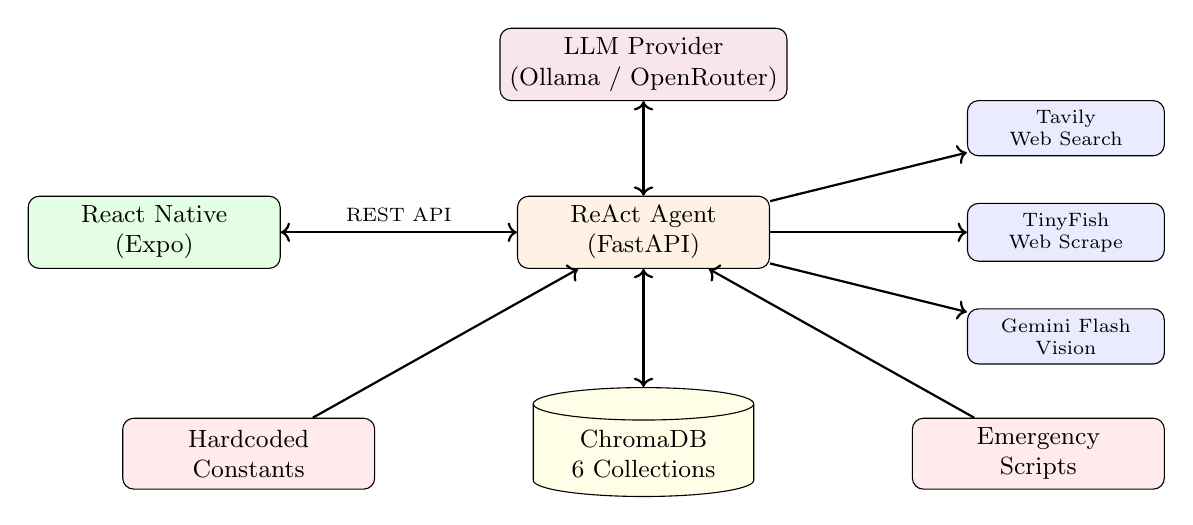
\begin{tikzpicture}[
    node distance=1.2cm and 2cm,
    box/.style={rectangle, draw, rounded corners=4pt, minimum width=3.2cm, minimum height=0.9cm, align=center, font=\small},
    dbbox/.style={cylinder, draw, shape border rotate=90, aspect=0.2, minimum width=2.8cm, minimum height=1cm, align=center, font=\small},
    apibox/.style={rectangle, draw, rounded corners=4pt, minimum width=2.5cm, minimum height=0.7cm, align=center, font=\scriptsize, fill=blue!8},
    arrow/.style={-{Stealth[length=2.5mm]}, thick},
]

\node[box, fill=green!10] (frontend) {React Native\\(Expo)};
\node[box, fill=orange!10, right=3cm of frontend] (agent) {ReAct Agent\\(FastAPI)};
\node[apibox, above right=0.5cm and 2.5cm of agent] (tavily) {Tavily\\Web Search};
\node[apibox, right=2.5cm of agent] (tinyfish) {TinyFish\\Web Scrape};
\node[apibox, below right=0.5cm and 2.5cm of agent] (vision) {Gemini Flash\\Vision};
\node[dbbox, fill=yellow!10, below=1.5cm of agent] (chroma) {ChromaDB\\6 Collections};
\node[box, fill=red!8, left=2cm of chroma] (constants) {Hardcoded\\Constants};
\node[box, fill=red!8, right=2cm of chroma] (emergency) {Emergency\\Scripts};
\node[box, fill=purple!10, above=1.2cm of agent] (llm) {LLM Provider\\(Ollama / OpenRouter)};

\draw[arrow, <->] (frontend) -- node[above, font=\scriptsize] {REST API} (agent);
\draw[arrow, <->] (agent) -- (llm);
\draw[arrow, <->] (agent) -- (chroma);
\draw[arrow, ->] (agent) -- (tavily);
\draw[arrow, ->] (agent) -- (tinyfish);
\draw[arrow, ->] (agent) -- (vision);
\draw[arrow, <-] (agent) -- (constants);
\draw[arrow, <-] (agent) -- (emergency);

\end{tikzpicture}
\caption{TripGuard system architecture. The ReAct agent orchestrates tool calls to the vector database, external APIs, and hardcoded data sources.}
\label{fig:architecture}
\end{figure}

\subsection{Technology Stack}

\begin{table}[H]
\centering
\begin{tabular}{@{}lll@{}}
\toprule
\textbf{Layer} & \textbf{Technology} & \textbf{Purpose} \\
\midrule
Frontend & React Native (Expo) & Cross-platform mobile app \\
Backend & FastAPI (Python) & REST API + agent loop \\
Vector DB & ChromaDB & Legal document retrieval \\
Embedding & BAAI/bge-m3 & Multilingual embeddings \\
LLM & Ollama / OpenRouter & Text generation (swappable) \\
Vision & Gemini 2.5 Flash & Traffic sign identification \\
Web Search & Tavily API & Real-time web fallback \\
Web Scrape & TinyFish API & Structured content extraction \\
Voice & ElevenLabs & Text-to-speech output \\
\bottomrule
\end{tabular}
\end{table}

\subsection{Agent Tools}

The agent has access to five tools and autonomously decides which to call:

\begin{itemize}[leftmargin=*]
    \item \textbf{\texttt{retrieve\_law}}: Semantic search over ChromaDB across 6 legal domains (traffic, drone, immigration, customs, narcotics, heritage). Called \textit{before every legal answer} - multiple times for cross-domain queries.
    \item \textbf{\texttt{lookup\_fine}}: Returns exact penalty amounts from a hardcoded table. The LLM is prohibited from generating fine numbers itself.
    \item \textbf{\texttt{get\_emergency\_steps}}: Returns offline-safe emergency scripts with step-by-step actions, hotlines, and embassy contacts.
    \item \textbf{\texttt{web\_search}}: Tavily search triggered when local corpus has insufficient coverage. Prioritizes trusted government sources.
    \item \textbf{\texttt{scrape\_url}}: TinyFish API to extract legal content from URLs found by \texttt{web\_search}.
\end{itemize}

\subsection{Retrieval Pipeline}

Retrieval follows a cascading strategy:

\begin{enumerate}[leftmargin=*]
    \item \textbf{Classify} the query into one of 6 legal domains via keyword matching (English + Vietnamese).
    \item \textbf{Vector search} within the target collection using BAAI/bge-m3 embeddings with a 0.55 cosine similarity threshold.
    \item \textbf{Fallback}: if $<$2 chunks pass the threshold, re-query across all collections.
    \item \textbf{Web fallback}: if local corpus is still insufficient, the agent calls \texttt{web\_search} $\rightarrow$ \texttt{scrape\_url} to get live information.
\end{enumerate}

\subsection{Legal Corpus}

Official Vietnamese legal documents were ingested from 6 domains:

\begin{itemize}[leftmargin=*]
    \item \textbf{Traffic}: NĐ 168/2024/NĐ-CP  -  \textbf{Drone}: NĐ 288/2025/NĐ-CP  -  \textbf{Immigration}: NĐ 07/2023/NĐ-CP
    \item \textbf{Customs}  -  \textbf{Narcotics} (Penal Code)  -  \textbf{Cultural Heritage}
\end{itemize}

Raw \texttt{.doc} files were processed with a custom parser handling the Word Binary Format's piece table structure and mixed encodings (UTF-16LE + CP1252), chunked at article (\textit{Điều}) granularity.

% ============================================================
\section{Key Features}
% ============================================================

\subsection{Nationality-Aware Responses}

During onboarding, users provide their nationality. The system automatically determines:

\begin{table}[H]
\centering
\begin{tabular}{@{}lccc@{}}
\toprule
& \textbf{Germany} & \textbf{USA} & \textbf{Japan} \\
\midrule
IDP valid? & Yes (Vienna 1968) & No (Geneva 1949) & Bilateral \\
Visa-free days & 45 & 0 (e-visa needed) & 45 \\
\bottomrule
\end{tabular}
\end{table}

The same question - ``Can I ride a motorbike?'' - yields a different answer per nationality.

\subsection{Hallucination Prevention}

LLMs hallucinate fine amounts. TripGuard prevents this structurally:
\begin{itemize}[leftmargin=*]
    \item Fine amounts are stored in hardcoded Python dictionaries sourced from official decrees.
    \item The agent \textit{must} call \texttt{lookup\_fine()} for any penalty - it cannot generate numbers.
    \item Every response cites the specific decree and article (e.g., ``NĐ 168/2024/NĐ-CP Điều 5'').
\end{itemize}

\subsection{Emergency Mode (Offline)}

Pre-authored scripts for 4 crisis scenarios, requiring zero internet:

\begin{itemize}[leftmargin=*]
    \item \textbf{Police stop}: What to show, what to say, max expected fine, how to request official receipt
    \item \textbf{Visa overstay}: Where to go, what to bring, fine amounts by duration
    \item \textbf{Drone confiscated}: How to cooperate, demand written receipt, embassy contact
    \item \textbf{Drug test positive}: Legal rights, embassy contact, what not to sign
\end{itemize}

\subsection{Traffic Sign Vision}

Upload a photo of a Vietnamese traffic sign $\rightarrow$ a vision-driven model identifies it per QCVN 41:2024 $\rightarrow$ agent retrieves the legal consequences of violating it.

% ============================================================
\section{Demo Flow}
\label{sec:demo}
% ============================================================

\begin{enumerate}[leftmargin=*]
    \item \textbf{Onboarding}: Select ``United States'' + motorbike rider + DJI Mini 4 Pro owner.

    \item \textbf{Checklist} (no API call - pure logic):
    \begin{itemize}
        \item[$\times$] US IDP (1949 Geneva) is invalid in Vietnam
        \item[$\times$] DJI Mini 4 Pro (895g) requires permit + Vietnamese org sponsor
        \item[$\times$] US citizens: 0 visa-free days, e-visa required
    \end{itemize}

    \item \textbf{Chat}: ``Can I ride a motorbike with my US license?''\\
    $\rightarrow$ \texttt{retrieve\_law(traffic)} $\rightarrow$ \texttt{lookup\_fine(no\_license)} $\rightarrow$ Illegal + 2--4M VND fine.

    \item \textbf{Multi-domain chat}: ``I want to fly my drone and ride a motorbike in Hội An''\\
    $\rightarrow$ \texttt{retrieve\_law(drone)} $\rightarrow$ \texttt{retrieve\_law(traffic)} $\rightarrow$ synthesized response covering both domains.

    \item \textbf{Vision}: Upload photo of a red circle sign $\rightarrow$ P.102 ``No Entry'' + violation fine.

    \item \textbf{Emergency}: ``Police stopped me'' $\rightarrow$ \texttt{get\_emergency\_steps()} $\rightarrow$ hardcoded step-by-step script, works offline.
\end{enumerate}

% ============================================================
\section{Future Work}
% ============================================================

\begin{itemize}[leftmargin=*]
    \item \textbf{Multi-country expansion}: Same architecture, new legal corpus - Thailand, Indonesia, and beyond.
    \item \textbf{Offline vector search}: Bundled compressed index for areas without internet.
    \item \textbf{Push alerts}: Notify users when regulations change during their trip.
    \item \textbf{Community layer}: Verified traveler reports layered on top of official legal data.
\end{itemize}

% ============================================================
\section{Conclusion}
% ============================================================

TripGuard combines RAG-grounded legal retrieval, hardcoded penalty data, and offline emergency scripts into a mobile assistant that protects foreign tourists from unintentional legal violations. By structurally separating verified facts from LLM-generated language, the system achieves the accuracy required for legal information while maintaining the accessibility of a natural language chatbot. The architecture is designed for straightforward extension to any jurisdiction - new country, new corpus, same system.

\begin{thebibliography}{00}

\bibitem{vnat2024} Vietnam National Administration of Tourism, ``International visitor arrivals to Viet Nam in December and 12 months of 2024,'' General Statistics Office of Vietnam, Dec. 2024. [Online]. Available: \url{https://vietnamtourism.gov.vn/}

\bibitem{vienna1968} United Nations Economic Commission for Europe, ``Convention on Road Traffic,'' Vienna, Nov. 8, 1968. Vietnam acceded in 2014.

\bibitem{tlalaw_idp} TLA Law Firm, ``IAA and IDP driving licenses: Which is valid in Vietnam for foreigners?'' 2024. [Online]. Available: \url{https://tlalaw.vn/iaa-and-idp-driving-licenses-which-is-valid-in-vietnam-for-foreigner.tla}

\bibitem{nd168} Government of Vietnam, ``Nghị định 168/2024/NĐ-CP quy định xử phạt vi phạm hành chính trong lĩnh vực giao thông đường bộ'' [Decree 168/2024/NĐ-CP on administrative penalties for road traffic violations], effective Jan. 1, 2025.

\bibitem{nd288} Government of Vietnam, ``Nghị định 288/2025/NĐ-CP quy định về quản lý tàu bay không người lái và các phương tiện bay khác'' [Decree 288/2025/NĐ-CP on management of unmanned aircraft and other aerial vehicles], Nov. 5, 2025.

\bibitem{nd07} Government of Vietnam, ``Nghị định 07/2023/NĐ-CP sửa đổi Nghị định 142/2021/NĐ-CP về xử phạt vi phạm hành chính trong lĩnh vực xuất nhập cảnh'' [Decree 07/2023/NĐ-CP on administrative penalties for immigration violations], 2023.

\bibitem{magesh2025} V. Magesh, F. Suber, N. Dye, J. Grant, and D. E. Ho, ``Hallucination-free? Assessing the reliability of leading AI legal research tools,'' \textit{Stanford Law School}, 2025.

\bibitem{dahl2024} M. Dahl, V. Magesh, M. Suzgun, and D. E. Ho, ``Large legal fictions: Profiling legal hallucinations in large language models,'' \textit{Journal of Legal Analysis}, vol. 16, no. 1, 2024.

\bibitem{yao2023react} S. Yao, J. Zhao, D. Yu, N. Du, I. Shafran, K. Narasimhan, and Y. Cao, ``ReAct: Synergizing reasoning and acting in language models,'' in \textit{Proc. ICLR}, 2023.

\bibitem{lewis2020rag} P. Lewis et al., ``Retrieval-augmented generation for knowledge-intensive NLP tasks,'' in \textit{Proc. NeurIPS}, 2020, pp. 9459--9474.

\bibitem{bge_m3} J. Chen, S. Xiao, P. Zhang, K. Luo, D. Lian, and Z. Liu, ``BGE M3-Embedding: Multi-lingual, multi-functionality, multi-granularity text embeddings through self-knowledge distillation,'' \textit{arXiv:2402.03216}, 2024.

\end{thebibliography}

\end{document}
